\section{\label{I-B-1}A musée d’exception, contraintes d’exception : un musée étroitement dépendant du ministère de la Défense. }

Bien qu'étant reconnu comme un musée de France au patrimoine exceptionnel, le \mae ne jouit pas d'une véritable autonomie. Dès sa naissance, il est en effet placé sous la tutelle du sous-secrétaire d'état à l'aéronautique militaire et maritime\footcite{terrierAeroportParisBourget2019}, et suit les évolutions de celui-ci lorsqu'il devient en 1928 le ministère de l'air, puis est rattaché au ministère de la Défense nationale en 1948. Aujourd'hui sous l'autorité du ministère des Armées, il est rattaché à la \gls{dmca}.


Tant du point de vue financier que culturel, le \mae dépend de politiques générales aux musées du ministère de l'Armée puisqu'il a une fonction de représentation de sa mémoire\footcite{museedelairetdelespaceProjetScientifiqueCulturel2020}. Il est donc pris dans un faisceau de décisions qui conditionnent ses évolutions techniques, documentaires ou institutionnelles : ainsi, jusqu'aux années 2000, agents et directeurs du musée étaient en grande partie issus du milieu militaire. Cette particularité de l'institution a pu contribuer à la création d'un décalage dans l'évolution de l'institution  par rapport à celle d'autres dont les agents seraient issus des professionnels des musées\footnote{Ceci ressort particulièrement lors des interviews auprès d'agents les plus anciens de l'institution, cf. Annexe \ref{Ax-D}. }. Cette impression généralisée au \ac{dsc} provient également du décalage inverse qui existe aujourd'hui, lorsque l'intégralité des agents du musée -- mis à part un officier de liaison -- sont issus du monde civil et ne partagent pas toujours la même culture que l'institution publique qu'ils représentent.

Concrètement, cette dépendance se traduit dans la difficulté éprouvée par le musée de mettre en place de nouveaux projets lorsqu'ils nécessitent des fonds exceptionnels ou une mise en place particulière. Le \mae appartient en effet à un vaste réseau de musées dépendant du ministère des Armées : de grands musées parisiens comme le musée de l'armée aux Invalides ou le musée de la Marine et ses 4 antennes en région, mais également des institutions plus petites comme le musée du Service de Santé des Armées au Val de Grâce ou celui du Génie à Angers
	\footnote{Voir \url{https://www.defense.gouv.fr/sga/memoire-culture-archives/culture/musees}}. 
Lors des missions qui ont été réalisées durant ce stage, ce sont surtout dans les choix d'outils informatiques de catalogage et de diffusion des collections que c'est ressentie cette contrainte. Les chantiers de mise en place de nouveaux logiciels qui se sont achevé cet été 2025 ont par exemple tous deux été pilotés par le ministère de la Défense : la mise en place du logiciel de gestion des collections \textit{Archange} (\textit{S/Museum} de \textit{Skinsoft}) s'inclut dans un projet progressif d'intégration des musées du ministère sur une même plateforme de gestion des collections. La migration vers le \ac{sigb} \textit{Koha} pour la bibliothèque, et la diffusion de ses collections sur la plateforme \textit{Clade} s'inscrit dans un projet similaire pour toutes les bibliothèques du ministère, afin d'unifier leur gestion mais aussi d'améliorer leur accessibilité en permettant à l'utilisateur d'interroger sur le même portail l'ensemble des \enquote{\textit{bib-musées}}.


	\begin{figure}[!]
		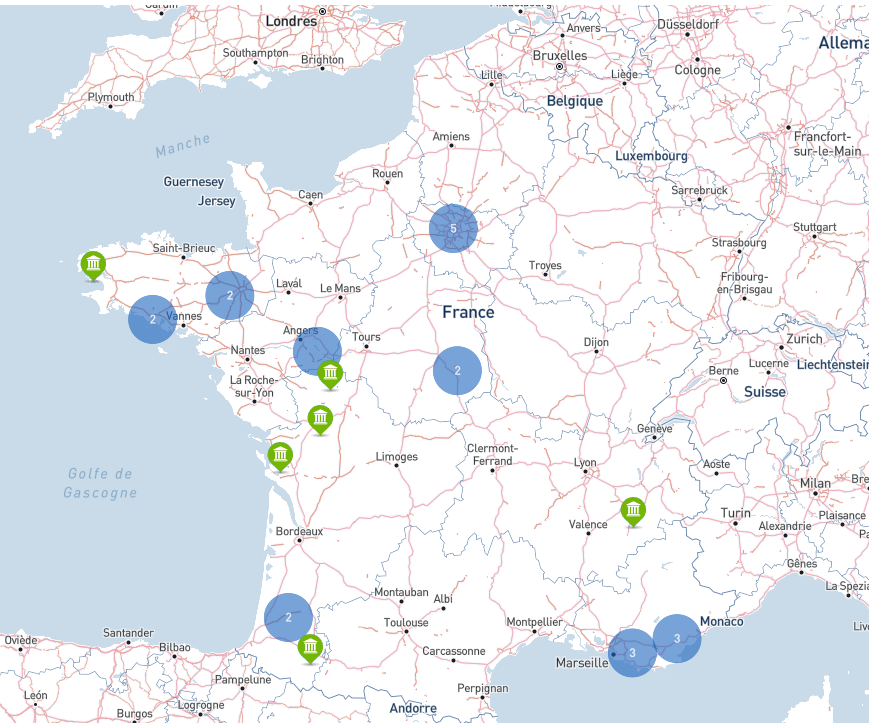
\includegraphics[width=\linewidth]{img/CART_musees_armee.png}
		\caption{De nombreux musées dépendent aujourd'hui du ministère des Armées (carte disponible sur \href{https://www.memoiredeshommes.sga.defense.gouv.fr/musees-collections-et-mecenat/musees-et-monuments}{Mémoire des hommes}).}
		\label{fig:cart_musees}
	\end{figure}


% 
%Ceci vaut donc autant pour les choix informatiques que pour les outils de catalogage ou de diffusion des collections. L’intégration d’un outil tel qu’Opentheso dans Koha, par exemple, ne saurait être envisagée sans considérer son impact sur l’ensemble des musées et bibliothèques relevant de la même tutelle. Le musée partage son infrastructure avec d'autres entités défendant un patrimoine militaire et technique, et c’est donc à l'échelle ministérielle que les décisions sont prises, parfois au prix d’une adaptation imparfaite aux besoins spécifiques du site du Bourget.\footnote{Par exemple, la cartographie des flux de données de thésaurus au \mae en Annexe \ref{Ax-C} montre bien le rôle central du ministère des armées comme validateur et gestionnaire des bases de données publiques du musée (Archange et Clade).}
%
%Ces décisions techniques sont également influencées par les priorités politiques du ministère, notamment en ce qui concerne la présence du musée dans les grands événements comme le salon du Bourget. L’ANSI (Agence du Numérique de la Sécurité Informatique) joue par ailleurs un rôle déterminant dans la validation des solutions techniques, imposant des contraintes de sécurité parfois difficilement conciliables avec les outils de la recherche ou du patrimoine. La gestion documentaire, l’interopérabilité des thésaurus, ou encore la diffusion des collections ne peuvent donc être pensées uniquement à léchelle du musée lui-même. À cela s’ajoute un panorama complexe de tutelles multiples : entre la Direction de la Mémoire, de la Culture et des Archives (DMCA), la Délégation à l’Information et à la Communication de la Défense (DICoD), et les directions propres à chaque arme, les marges de manœuvre apparaissent étroites.
%
